\chapter{Method}

\section{Choice of Method}


\begin{figure}[h]
%\hspace*{-0.4cm}
\begin{center}
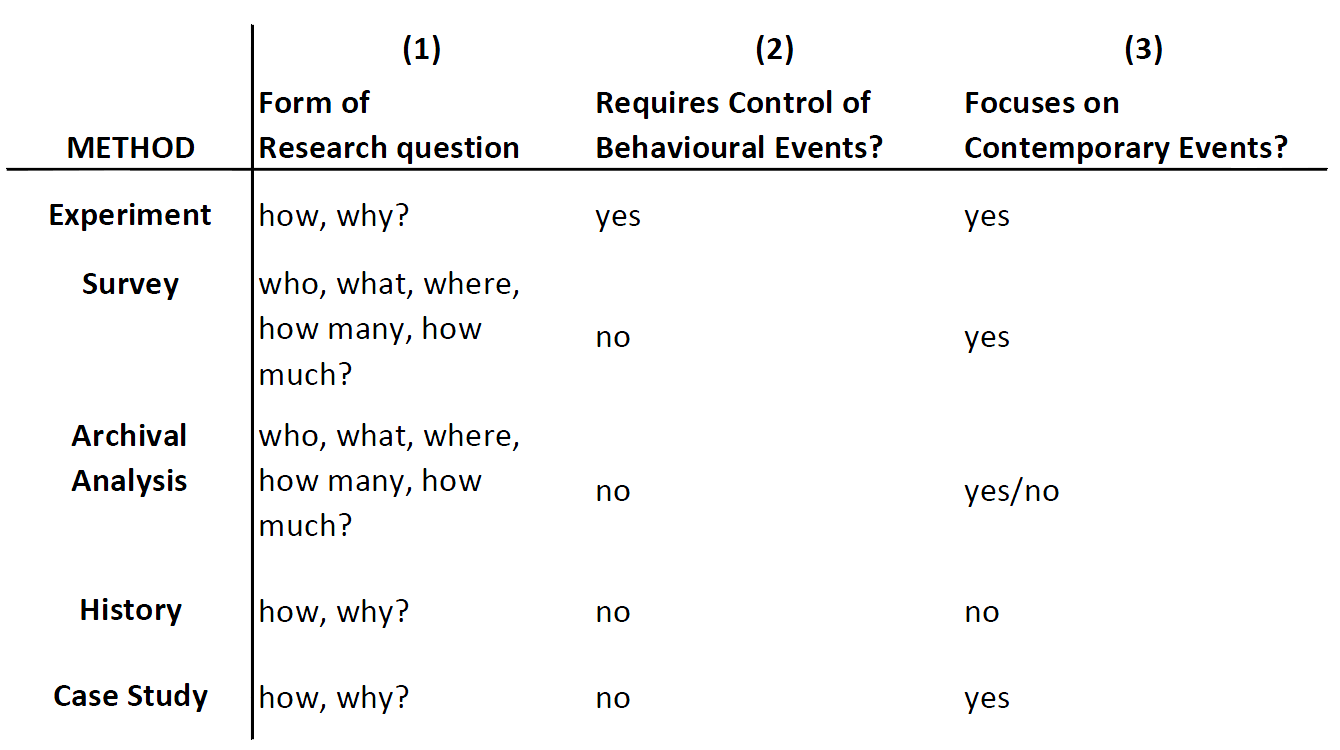
\includegraphics[scale=0.35]{methods.png}
\caption[Situations for different research methods]{Situations for different research methods, derived from \cite{CaseStudyResearch}}
\label{fig:methods}
\end{center}
\end{figure}

  

\section{Case Study}

%\cite{CaseStudyResearch}
%\cite{kitchenham1995case}
\subsection{Background Study}

\subsection{Interviews}

qualitative vs quantitative
qualitative eliminated the possibility to generalize the results. We chose to do semi-structured interviews conducted face-to-face.   




For the interviews in our study we chose a qualitative approach. \cite{cassell2004essential} states that the goal of qualitative interviews is to see the research topic from the interviewee's perspective and understand why and how they got that particular perspective. To enable this, qualitative interviews are driven by open questions and a low degree of structure. Questions focus on specific situations and experiences made by the interviewee. 

We define the interviews as semi-structured. Our purpose was to get the interviewee to talk freely about their experiences. We needed to have a list of questions prepared to ensure we got all the information required to answer our research questions, however. In addition to our predefined questions, we also had the opportunity to ask follow-up questions. By performing interviews this way, the interviewee can be seen as a ``participant" in the research, rather than an object just answering pre-defined questions given by the interviewer.




Prior to choosing this method of study, we weighted pros and cons. We concluded an qualitative approach to our research were the most convenient(time?) and interesting.
 
%advantages
\paragraph{Flexible} By choosing this method



%disadvantages
\paragraph{Time-Consuming} Developing an interview guide, carrying out interviews and analysing them can be highly time-consuming activities. Participating in interviews is also time-consuming for interviewees, which could make it challenging to recruit interviewees for our study. One approach to mitigate the risk of not recruiting interviewees for our study was sending out letters explaining the main purpose of the study, what was expected by the interviewee, and how the interviews would play out. We also notified organizations at an early stage and set dates for the interviews to ensure their commitment.

\paragraph{Practical issues} 

\subsection{Document study}
%\subsection{Action Research}

\section{Ethical Considerations}
%Litt i forhold til at man behandler sensitiv information og sånn
\subsection{Anonymization}

\section{Challenges}